\graphicspath{{03-Ckov/Figures/}}

\section{Cherenkov Detectors}
\label{Sect:Ckov}

The threshold Cherenkov counters were designed primarily to provide
$\pi$-$\mu$ separation for particle momentum~$\gsim 200$\,MeV/$c$, where
the precision of the time-of-flight measurement was not sufficient for
conclusive particle identification.
Two high-density silica aerogel Cherenkov detectors with refractive
indices $n$=1.07 (CkovA) and $n$=1.12 (CkovB) were
used~\cite{Cremaldi:2009zj}.
The structure of the detectors is shown in ~figure~\ref{fig:ckov1}.
Light was collected in each counter by four eight-inch, UV-enhanced
PMTs and recorded using CAEN V1731 FADCs (500\,MS/s)~\cite{NOTE473}.
The two detectors were placed directly one after the other in the
beamline and located just after TOF0.

The refractive indices of CkovA and CkovB result in detection
thresholds for muons of approximately 280\,MeV/$c$ and 210\,MeV/$c$ respectively.
For pions the thresholds are approximately 367\,MeV/$c$ (CkovA) and
276\,MeV/$c$ (CkovB).
MICE was designed to operate using beams with a central momentum
between 140\,MeV/$c$ and 240\,MeV/$c$.
%The thresholds of CkovA and CkovB were chosen to match this range
%since the TOF system was able to identify muons with high efficiency
%for momenta below 210\,MeV/c.
%For momentum greater than 210\,MeV/c and less than 276\,MeV/c, above
%the maximum beam momentum, muons will produce a signal in CkovB while
%pions will produce no signal in either detector.
The Cherenkov counters thresholds were chosen to provide muon identification for beams of 210\,MeV/$c$ and above, while the TOFs provide muon identification for beam less  than 210\,MeV/$c$.
Unambiguous identification of particle species using the Cherenkov
exploited the momentum measurement provided by the trackers. \\
\begin{figure}
  \begin{center}
    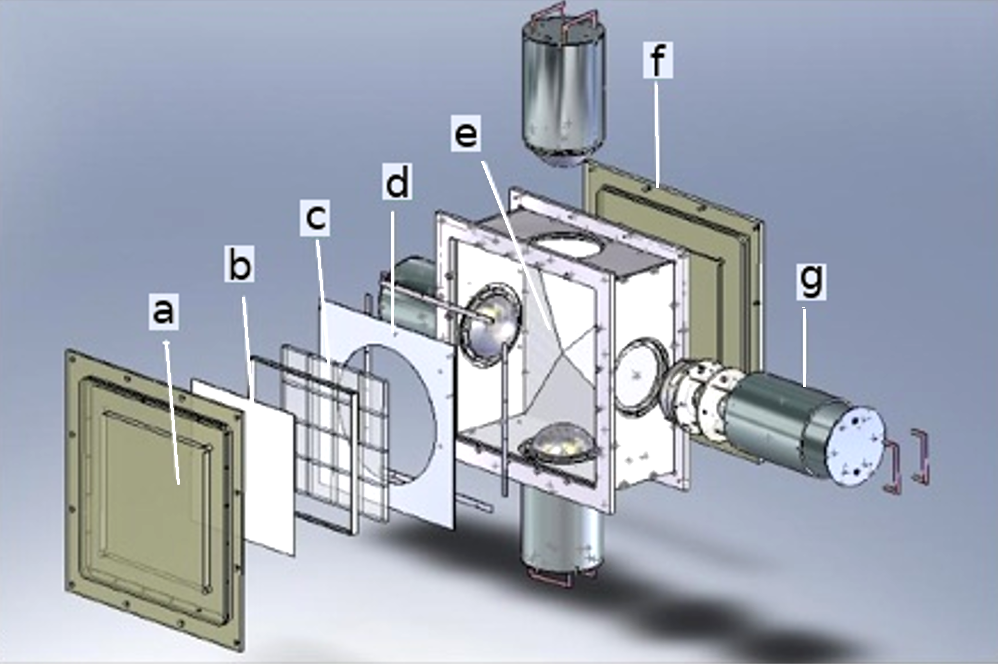
\includegraphics[width=0.6\columnwidth]{./03-Ckov/Figures/Ckov_fix.png}
  \end{center}
  \caption{
    MICE aerogel Cherenkov counter: a)~entrance window,
    b)~mirror, c)~aerogel mosaic, d)~acetate window, e)~GORE reflector
    panel, f)~exit window and g)~eight-inch PMT in iron shield.
  } 
  \label{fig:ckov1}
\end{figure}

\noindent\textbf{Performance} \\
\noindent
The performance of the detectors was determined using beams for which
the momentum range was broad enough to observe the turn-on point and to
allow the asymptotic light yield (as the particle velocity divided by the speed of light, $\beta$, approaches 1) to be
obtained from a fit to the data.
The normalised photo-electron yields observed in CkovA and CkovB are
plotted as a function of $\beta\gamma$ (where $\gamma=(1-\beta^2)^{-1/2}$) in
figure~\ref{fig:ckov_betagamma}.
The pedestal in the photo-tube response arising from background
photons has been subtracted.
The approximate turn-on points for CkovA and CkovB were found at
$\beta\gamma \approx 2.6$ and $\approx 2.1$ respectively,
corresponding to refractive indices of $n \approx 1.07$ and $\approx 1.11$ which are in broad agreement with the
properties of the aerogel radiators. 
\begin{figure}
  \begin{center}
    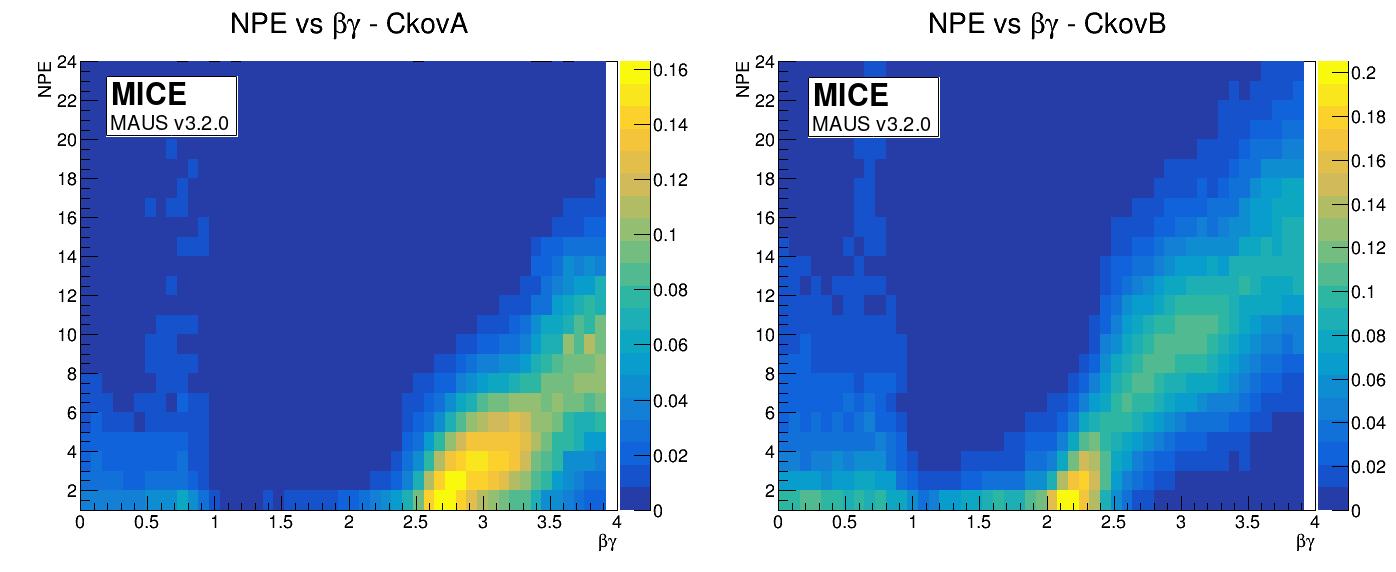
\includegraphics[width=0.90\columnwidth]{./03-Ckov/Figures/scatter_betagamma_logo.png}
    \caption{Photoelectron yields versus $\beta\gamma$ in CkovA and CkovB.}
    \label{fig:ckov_betagamma}
  \end{center}
\end{figure}
